% !TEX TS-program = pdflatex
% !TEX encoding = UTF-8 Unicode

% This is a simple template for a LaTeX document using the "article" class.
% See "book", "report", "letter" for other types of document.

\documentclass[11pt]{article} % use larger type; default would be 10pt.
\setcounter{secnumdepth}{2}

\usepackage{paralist} % very flexible & customisable lists (eg. enumerate/itemize, etc.)

\usepackage{hyperref}

\usepackage[utf8]{inputenc} % set input encoding (not needed with XeLaTeX)
\usepackage{float} % to place float images correctly
\usepackage{color} % to color text
\usepackage{enumitem} % for lists
\usepackage{subfigure} % for mockups
\usepackage[font={it}]{caption} % for captions


%%% Examples of Article customizations
% These packages are optional, depending whether you want the features they provide.
% See the LaTeX Companion or other references for full information.

%%% PAGE DIMENSIONS
\usepackage{geometry} % to change the page dimensions
\geometry{a4paper} % or letterpaper (US) or a5paper or....
% \geometry{margin=2in} % for example, change the margins to 2 inches all round
% \geometry{landscape} % set up the page for landscape
%   read geometry.pdf for detailed page layout information

\usepackage{graphicx} % support the \includegraphics command and options

% \usepackage[parfill]{parskip} % Activate to begin paragraphs with an empty line rather than an indent

\usepackage{listings}
\usepackage{color}
 
\definecolor{codegreen}{rgb}{0,0.4,0}
\definecolor{codegray}{rgb}{0.5,0.5,0.5}
\definecolor{codepurple}{rgb}{0.58,0,0.82}
 
\lstdefinestyle{mystyle}{ 
    commentstyle=\color{magenta},
    keywordstyle=\color{blue}\bfseries,
    numberstyle=\tiny\color{codegray},
    stringstyle=\color{codepurple},
    basicstyle=\footnotesize,
    breakatwhitespace=false,         
    breaklines=true,                 
    captionpos=b,                    
    keepspaces=true,                 
    numbers=left,                    
    numbersep=5pt,                  
    showspaces=false,                
    showstringspaces=false,
    showtabs=false,                  
    tabsize=2,
   emph={self}, 
   emphstyle=\color{blue}, 
   emph={[2] BookingManager, FineManager}, 
   emphstyle=[2]\color{codegreen}\bfseries, 
   emph={[3]__init__, newBook, removeReservation, getReservation, manageExpired, min_heap, pop, now, timedelta, expireReservation}, 
   emphstyle=[3]\color{codegreen}, 
}
 
\lstset{style=mystyle}





%%% PACKAGES
\usepackage{booktabs} % for much better looking tables
\usepackage{array} % for better arrays (eg matrices) in maths
%\usepackage{paralist} % very flexible & customisable lists (eg. enumerate/itemize, etc.)
\usepackage{verbatim} % adds environment for commenting out blocks of text & for better verbatim
%\usepackage{subfig} % make it possible to include more than one captioned figure/table in a single float
% These packages are all incorporated in the memoir class to one degree or another...

%%% HEADERS & FOOTERS
\usepackage{fancyhdr} % This should be set AFTER setting up the page geometry
\pagestyle{fancy} % options: empty , plain , fancy
\renewcommand{\headrulewidth}{0pt} % customise the layout...
\lhead{}\chead{}\rhead{}
\lfoot{}\cfoot{\thepage}\rfoot{}

%%% SECTION TITLE APPEARANCE
\usepackage{sectsty}
\allsectionsfont{\sffamily\mdseries\upshape} % (See the fntguide.pdf for font help)
% (This matches ConTeXt defaults)

%%% ToC (table of contents) APPEARANCE
\usepackage[nottoc,notlof,notlot]{tocbibind} % Put the bibliography in the ToC
\usepackage[titles,subfigure]{tocloft} % Alter the style of the Table of Contents
\renewcommand{\cftsecfont}{\rmfamily\mdseries\upshape}
\renewcommand{\cftsecpagefont}{\rmfamily\mdseries\upshape} % No bold!

\newcommand{\pe}{PowerEnJoy }
\newcommand{\pecomma}{PowerEnJoy, }
\newcommand{\bul}[1]{\indent$\bullet$ #1\\}

\usepackage{listings}
\usepackage{pxfonts}
\usepackage{enumitem}
\usepackage{tabularx}
\usepackage{pdfpages}


\newcommand{\extInput}[3]{ #1:  \textbf{#2} \\ #3  }


%%% END Article customizations

%%% The "real" document content comes below...




\title{Project Planning Document}
\author{Simone Mosciatti \& Sara Zanzottera}

\begin{document}
\maketitle
\newpage
\tableofcontents
\newpage


\section{Introduction}

\subsection{Purpose and Scope}

The main purpose of this Project Plan Document is to assess the expected complexity of \pecomma, evaluate the risks related to the project, estimate costs and effort we expect will be required in order to develop our software successfully.

This document is also meant to provide some guidelines for the project manager to allocate budget and resources to the project, and to help defining a schedule for the development team.

We are using Function Points and COCOMO II analysis to estimate the size of the project, in terms of lines of code and costs and effort required to get the final product in time. 

Then we provide a tentative schedule and a Gantt covering all the activities required to complete the project, from the very first operation to the actual deployement, that should help the managers defining a schedule. We also describe the expected load allocation for the team members.

Finally we provide a risk analysis for the most probable setbacks the project may face, and provide some preventive measures that should be performed in order to prevent a later, not recoverable failure in providing a software matching the expectations, in terms of feature, quality of code, costs and timing.


\subsection{Definitions, Acronyms, Abbreviations}
 \begin{description}
	\item[RASD] Requirements and Specification Document.
	\item[DD] Design Document.
	\item[User] A customer of \pe using the service.
	\item[Staff Operator (Operator)] An employee of \pe which takes care of the cars.
	\item[Ride] The action of getting onboard of a \pe car, start its engine, drive to destination and park.
	\item[Issue] Any problem a car may incur in, or a user may face while using the service.
	\item[Nearby Cars] Available cars located within a maximum distance to a specific position.
	\item[Available Cars] Cars whose Availability Status is set to ``Available``.
	]\item[Booking (Reservation)] The act to reserve a car for a limited amount of time for future use by a user.
	\item[Driver] Whoever is driving a regularly booked \pe car.
	\item[Driving License] The state's issued driving license of the user.
	\item[Fine] A fine issued by the local law enforcing officers to a user while driving a \pe car. 
	\item[Safe Area] An parking area, predefined by the company, where is possible to safely park the cars of the \pe fleet.
	\item[Car's Onboard System] The controll system of the car that is able to exchange data with the central system and to relevate operation parameters.
	\item[Customer's App] An implementation of the system frontend tailored to the need of the customers.
	\item[Staff's App] An implementation of the system frontend tailored to the need of the staff.
	\item[Central System (Main Server)] The central system for \pe. All the command and all the data are streamed, analyzed and used here.
	\item[GPS]: Global Positioning System is a global navigation satellite system (GNSS) that provides location and time information in all weather conditions, anywhere on or near the Earth where there is an unobstructed line of sight to four or more GPS satellites.
	\item[Location] Pair of integer values as provided by GPS sensors.
	\item[Payment Method] Set of data relative to a credit card.
	\item[Identity ID] Personal code provided by local authorities to uniquely identify citizens.
	\item[Driving License ID] The unique code reported on every legal driving license.
	\item[Scanned License] An high quality image of the driving license acquired by the car's onboard system.
	\item[FP] Function Points.
	\item[ILF] Internal logic file
	\item[ELF] External logic file.
	\item[DBMS] Database Management System.
	\item[API] Application Programming Interface.
	\item[UI] User Interface.
  \end{description}

\subsection{Reference Documents}
\begin{itemize}
	\item \textit{Assignments AA 2016-2017.pdf} (Assignments document given by the teacher)
	\item \textit{Reqiurements And Specification Document} (referring to this project)
	\item \textit{Design Document} (referring to this project)
	\item	Reference for Functional Point \url{https://web.archive.org/web/20160516160212/http://www.softwaremetrics.com/fpafund.htm}
  \end{itemize}

\section{Project size, cost and effort}

\subsection{Size estimation}

Here we use the Function Point Approach to determine the size of the project.

Since we already have well defined components and the interaction of those components between external and internal actors, it seems natural to use the complexity of their interactions to determinate the Function Points for each component.

Provided that all the components have an intrisic, similar complexity, it is reasonable to assume that components that interact with few other components are quicker and simpler to develop. In our opinion the real complexity lies in the connection of components, not in the components themselves.

The complexity weights we use from now on are the following:
\begin{table}[h]
\centering
\bgroup
\def\arraystretch{1.5}%  1 is the default, change whatever you need
	\begin{tabular}{| c | c | c | c |}
	\hline
	Function Type & LOW & AVERAGE & HIGH \\
	\hline
	Internal Logical Files & 7 & 10 & 15 \\
	External Interface Files & 5 & 7 & 10 \\
	External Input & 3 & 4 & 6 \\
	External Inquiry & 3 & 4 & 6 \\
	External Output & 4 & 5 & 7 \\
	\hline
	\end{tabular}
\egroup
\caption{Function Point's complexity weights}
\end{table}


\subsection{Internal Logical Files}

All the internal files are stored in a database.

The model for our database was discussed in the Design Document, but we report again the diagram to simplify the discussion.

\begin{figure}[H]
	\centering
	\includegraphics[width=1\textwidth]{../Architecture/UML/ModelZoomComponents.png}
	\caption{Class Diagram of the Model.}
\end{figure}	

We are considering all the components of LOW complexity except for:
\begin{itemize}[noitemsep]
	\item BOOKING entity: HIGH complexity. it is the central entity in the whole application, with a lot of relationships with other components and very high insert rates.
	\item CAR entity: AVERAGE complexity. It has a relationship with BOOKING, but has a lot of very volatile fields and its update rates are very high.
\end{itemize}

\subsubsection{Total for IFL}
Total = 8 * 7 + 10 + 15 =  81


\subsection{External Interface Files}

The project involves 3 external data sources.

\begin{description}
	\item[stripe] We consider this service of AVERAGE complexity. They provide a very extensive set of endpoints, but the documentation is extremelly well done. In addition, we need to use only a small subset of the available endpoints and they provide several facilities to test the integration seamlessly.
	\item[linfo.io] We consider this service of LOW complexity. Its only end point requires two inputs (center of the circle and radius) and return a set of objects inside that circle.
	\item[truelicense.com] We consider this service of LOW complexity. Its APIs consist of only one single endpoint where to send an image, providing in output the number of the license of the input image, if valid.
\end{description}

\subsubsection{Total for EIF}
Total = 7 + 5 + 5 = 17

\subsection{External Input}

Following the list of functionalities provided in the Design Document, we identified the following External Input sources and assessed their complexity.

\subsubsection{USER Component}


\begin{description}
	\item \extInput
		{USER/Register}
		{AVERAGE}
		{Some information need to be validated and it is necessary to be sure of the uniqueness of the users.}
	\item \extInput
		{USER/\{Login/Logout\}}
		{LOW}
		{Only few check are necessary to LOG a user, such a validate the credentials.}
	\item \extInput
		{USER/SetPaymentMethod}
		{AVERAGE}
		{It is necessary to coordinate the changes with the external system of paymet (stripe).}

\end{description}

\subsubsection{GEOLOCATION Component}

\begin{description}
	\item \extInput
		{GEOLOCATION/AvailableCar}
		{HIGH}
		{It handle geolocation queries. Its complexity should be AVERAGE, but we will put more effort in developing general routines in order to lower the complexity of all the other functionality that requires geolocation queries.}
	\item \extInput
		{GEOLOCATION/Areas}
		{LOW}
		{We can reuse many routines from GEOLOCATION/AvailableCar to build this function with a minimum effort. On top of that, most of this work is delegate to the external service linf.io}
	\item \extInput
		{GEOLOCATION/Issues}
		{LOW}
		{We can reuse many routines from GEOLOCATION/AvailableCar to build this function with a minimum effort.}
	\item \extInput
		{GEOLOCATION/IsSafeArea}
		{LOW}
		{We can reuse many routines from GEOLOCATION/AvailableCar to build this function with a minimum effort.}

\end{description}

\subsubsection{POSITION Component}

\begin{description}
	\item \extInput
		{POSITION/Car}
		{AVERAGE}
		{This function requires the use of the car's onboard system and the communication system.}
	\item \extInput
		{POSITION/User}
		{LOW}
		{This function uses the GPS inside the user device, however it is a pretty standard, well known function.}
	\item \extInput
		{POSITION/Areas}
		{LOW}
		{Little more than a simple lookup in the database}
\end{description}

\subsubsection{BOOKING Component}

\begin{description}
	\item \extInput
		{BOOKING/Book}
		{LOW}
		{A simple write operation in the database. Most of the consistency checks are handled by the DBMS itself.}
	\item \extInput
		{BOOKING/Unbook}
		{LOW}
		{A simple update in the database. Most of the consistency checks are handled by the DBMS itself.}
	\item \extInput
		{BOOKING/Expire}
		{AVERAGE}
		{Other than modifying the database, this functionality needs to interact with the external payment system.}
\end{description}

\subsubsection{CAR Component}

\begin{description}
	\item \extInput
		{CAR/Unlock}
		{LOW}
		{Provided a reliable channel of communication with the car and a working on board system (assumption that I will keep for the rest of the documet), this functionality is a simple request to the car on board main system.}
	\item \extInput
		{CAR/ValidateLicense}
		{LOW}
		{Most of the work is handled by the external component truelicense.com}
	\item \extInput
		{CAR/Lock}
		{AVERAGE}
		{It is a simple command send to the car on board system. However, it has to trigger correctly the payment procedure starts.}
	\item \extInput
		{CAR/TurnOff}
		{LOW}
		{It is a simple command send to the car on board system.}
	\item \extInput
		{CAR/Telemetry}
		{HIGH}
		{By itself this component should have a LOW complexity. However, assigning a HIGH complexity we are considering the complexity of setting up a reliable communication channel between the main server and the cars.}
	\item \extInput
		{CAR/SetStatus}
		{LOW}
		{It is a simple update in the database.}
	\item \extInput
		{CAR/GetDetails}
		{LOW}
		{It is a simple read in the database. If data is too old, it also involves some communication from the server to the car, an operation still considered of LOW complexity.}
\end{description}

\subsubsection{RIDE Component}

\begin{description}
	\item \extInput
		{RIDE/Start}
		{LOW}
		{It simply performs an update in the database.}
	\item \extInput
		{RIDE/End}
		{LOW}
		{It simply performs an update in the database.}
\end{description}

\subsubsection{ISSUE\_MANAGER Component}

\begin{description}
	\item \extInput
		{ISSUE/New}
		{LOW}
		{It simply performs an update in the database.}
	\item \extInput
		{ISSUE/TakeCharge}
		{LOW}
		{It simply performs an update in the database.}
	\item \extInput
		{ISSUE/Solve}
		{LOW}
		{It simply performs an update in the database.}
	\item \extInput
		{ISSUE/GiveUp}
		{LOW}
		{It simply performs an update in the database.}
\end{description}

\subsubection{Total for Externa Input}
Total = 18 * 3 + 6 * 6 + 2 * 6 =  102

\subsection{External Inquiry}

\subsubsection{RIDE\_MANAGER Component}
\begin{description}
	\item \extInput
		{RIDE/FindRides}
		{LOW}
		{It is a simple lookup in the database.}
\end{description}

\subsubsection{Total for External Inquiry}
Total = 1 * 3 = 3

\subsection{External Output}

\subsubsection{BILLING\_MANAGER Component}
\begin{description}
	\item \extInput
		{BILL/CalculateRideFee}
		{AVERAGE}
		{It require to know the overall time of the ride and the bonus and malus applied.}
	\item \extInput
		{BILL/CalculateExpireBookFee}
		{LOW}
		{It returns a constant value.}
	\item \extInput
		{BILL/CalculateUnsafeParkingFine}
		{LOW}
		{It returns a constant value.}
\end{description}

\subsubsection{NOTIFIER}
\begin{description}
	\item \extInput
		{NOTIFY/Notify}
		{AVERAGE}
		{This functionality takes care of different types of notification. It is not ``a size fits all''.}
\end{description}

\subsubsection{Total for External Output}
Total = 2 * 4 + 2 * 5 = 18

\subsection{Overall count}

The overal total is: \hfill
81 + 17 + 102 + 3 + 18 = 221

Which provide a lower bound of roughly:\hfill
221 * 46 = 10166

and an upper bound of: 
\hfill
221 * 67 = 14807

lines of code.

\section{Cost Estimation COCOMO II}

In this section we are exploring the scale and the cost drivers for the COCOMO II model in order to find a reasonable time of execution of the project.

\subsection{Scale Driver}

Given the table in the reference, we attribute the following values to the Scale Driver.

\begin{description}
	\item[PREC] Precedentedness: The team is Generally familiar with the problem space, it has never built the same product before but it has build several part of it a lot of time. 2.48
	\item[FLEX] Development Flexibility: All the documents are been written with the assumption that during the development phase a lot of unforanseeable issues would arise, we are expecting general conformity of the finished product to the designed one. 2.03
	\item[RESL] Architecture / Risk Resolution: In the following part of the document we present a quite comprensive risk mitigation strategy. 2.83
	\item[TEAM] Team Cohesion: The team is highly cooperative. 1.10
	\item[PMAT] Process Maturity: The team already works in the industry and know and apply best practise. 3.12
\end{description}

\subsection{Cost Driver}

\begin{description}
	\item[RELY]: Required Software Reliability: In case of the interuption of the service there won't be heavy financial losses, but only easible recoverble losses: 1.00
	\item[DATA]: Data Base Size: 	Our most populated table will have less than 100k rows for the foreaseble future, given the lower bound of roughly 10k SLOC our D/P ratio is of less than 10: n/a
	\item[CPLX]: Product Complexity: Our code does not present any over complex structure, we will set to nominal the overall complexity: 1.00
	\item[RUSE]: Developed for Reusability: We will develop for reusability across the project: 1.00
	\item[DOCU]: Documentation Match to Life-Cycle Needs: We will definitely keep the documentation in sync with the release of the application: 1.00
	\item [TIME]: Execution Time Constraint: The software is not particulary CPU bounded, overall we are expecting a fairly low use of CPU: 1.00
	\item[STOR]: Main Storage Constraint: Storage is definitely not an issue nowadays: n/a
	\item[PVOL]: Platform Volatility: We are going to base all our stack on prooven and used open source components, we are conservatevely setting this value to nominal: 1.00
	\item[ACAP]: Analyst Capability: We are confident that we conduct a fairly comprensive analysis of the overall project and so we set this value to high: 0.85
	\item[PCAP]: Programmer Capability: We both have real word experince working in complex project and in contributing to the open source: 0.88
	\item[PCON]: Personnel Continuity: There will be no turnover: 0.81
	\item[APEX]: Applications Experience: We have choose technologies that we know and that we have already used: 0.88
	\item[PLEX]: Platform Experience: Again we have choose the platform based on our previous experience: 0.91
	\item[LTEX]: Language and Tool Experience: We both have worked before with all the tools that we will need in the project and as well with the languange: 0.91
	\item[TOOL]: Use of Software Tools: We are going to automate as much as possible of the whole lifecycle of the product: 0.90
	\item[SITE]: Multisite Development: The team will be located in the same city and will use all the technology to communicate as much as possible: 0.86
	\item[SCED]: Required Development Schedule: We don't plan to inpose any schedule constraint on the project: 1.00
\end{description}

Overall the result of the analysis of the cost driver is the following:

\begin{tabular}{| c | c | c | c |}
\hline
RELY & Precedentedness & Nominal & 1.00 \\ \hline
DATA & Development Flexibility & Very Low & n/a \\ \hline
CPLX & Product Complexity & Nominal & 1.00 \\ \hline
RUSE & Developed for Reusability & Nominal & 1.00 \\ \hline
DOCU & Documentation Match to Life-Cycle Needs & Nominal & 1.00 \\ \hline
TIME & Execution Time Constraint & Nominal & 1.00 \\ \hline
STOR & Main Storage Constraint & Low & n/a \\ \hline
PVOL & Platform Volatility & Nominal & 1.00 \\ \hline
ACAP & Analyst Capability & High & 0.85 \\ \hline
PCAP & Programmer Capability & High & 0.88 \\ \hline
PCON & Personnel Continuity & Extra High & n/a \\ \hline
APEX & Applications Experience & High & 0.88 \\ \hline
PLEX & Platform Experience & High & 0.91 \\ \hline
LTEX & Language and Tool Experience & High & 0.91 \\ \hline
TOOL & Use of Software Tools & High & 0.90 \\ \hline
SITE & Multisite Development & Very High & 0.86 \\ \hline
SCED & Required Development Schedule & Nominal & 1.00 \\ \hline \hline 
\multicolumn{3}{| c |  }{Product} & 0,422 \\ \hline
\end{tabular}

\section{Effort Estimation}

Given the above point we can estimate the effort in Person-Month (PM).

We will use the following formula:

Effort = A * EAF * KSLOC \^ E

Using the following substitution:

A = 2.94

EAF = 0.422 

E = B + 0.01 sum(scale driver) = 0.91 + 0.01 * 11.56 = 0.91 + 0.1156 = 1,0256

Lower Bound = 2.94 * 0.422 * 10.166 ** 1.0256 = 13.38

Upper Bound = 2.94 * 0.422 * 14.807 ** 1.0256 = 19.68

Duration = 3.67 * Effort ** F \\

F = 0.28 + 0.2 * (E - B) = 0.28 + 0.2 * (1.0256 - 0.91) = 0.303

DurationLower = 3.67 * 13.38 ** 0.303 = 8.05

DurationUpper = 3.67 * 19.68 ** 0.303 = 9.05


\section{Schedule}

Given that most of the analysis is already done in this project we are going to focus on the scedule of the development and the deployement of the software.

Because of our risk mitigation strategy there will be need to validate the product as early as possible, this will impose slower development cycles but we will be more sure about what the final result will be also from a bussiness perspective, we can afford this since our time estimetion are quite short. Nevertheless we are still accounting for an additional two month of time, bringing the total time of development to roughly 11 moths.

We believe that this is a reasonable tradeoff, between the use of time and the risk management.

We will start developing a very simple MVP where selected alpha user will be able to rent cars once a day for a small nominal fee. The manual selection of the user will avoid that the car will be damaged or that they will abuse of the system, at the same time will provide us with extremelly valuable feedback on the system we are building and the interaction with the users.

During the MVP phase techinical staff will be always present in order to manually fix any kind of problem that may arise.

After this phase, if the stackholder of the project agree to proceed, we will start the creation of the real platform.

We will decide what part of the MVP keep (if any), anyway the experience gained build the MVP will be extremelly valuable in this phase, and will let us move very fast with confidence. 
During this phase we will develop also the unit and the integration test.

We will keep a clean building/deploy pipeline so that we will always able to deploy our platform.

Keeping such pipeline will be expensive and time consuming but it will provide a lot of benefits.

\begin{enumerate}
	\item Mirror the alpha traffic to the new service
	\item Slowly move the alpha user to the new service and effectively make then beta user
	\item Slowly add more beta user to the service
\end{enumerate}

Using this approach the developing time will be longer but we are keeping the risk as low as possible, we can afford this since our design is extremely decouple and simple to build, so our developing time are short.

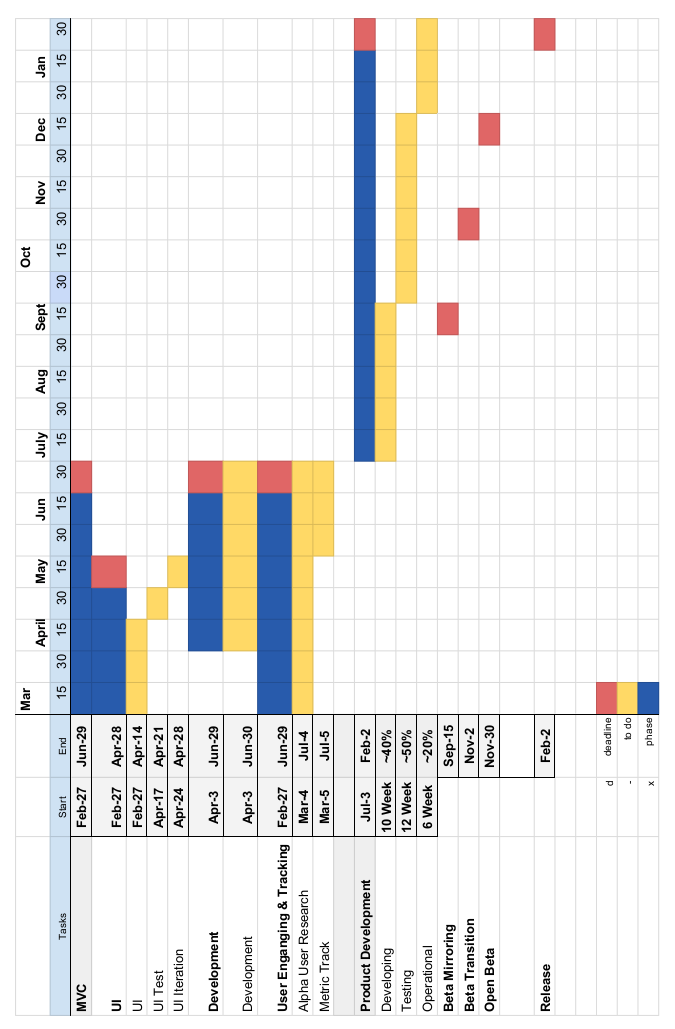
\includepdf[]{GANTT/GANTT}

In the above Gantt chart we avoided to actually specify what time slot is associated with what activity, but we simply give an estimation about the percentage of time the development activity should take of the whole time period.

This is required since all the activity on each module should procede in parallel with developing and test well complected and the setting of the operational activity shortly after.

Using these methodology will let us incorporate the feedback from both the user and the test environment as soon as possible.

Ex. We may discover that the user will pay to book a car for more time than a single hour, using our methodology we will be able to incorporate such feedback immediately in the system.
Ex. We discover that some of our module is not able to keep up with the expected load we could immediately allocate more resources and time to that part.

\section{Resource Allocation}

Our small team has different and complementary skill.

Sara is more experienced in UI / UX and clearly communicate with the stackholder of the project; Simone is more experience in back end developing and M2M communication.

Both have a fairly good generic programming experience.

Since the components are already defined, as well their interface, only a single developer will be responsable for a component.

To fairly allocate the several component to the developers we will use the complexity factor calculate above.

Given the different experience of the developin team the two developer are allocate to the different modules in the following way:

\begin{description}
	\item[Simone] \hfill
		\begin{enumerate}
			\item GEOLOCATION
			\item POSITION
			\item CAR
			\item RIDE
		\end{enumerate}
	\item[Sara] \hfill
		\begin{enumerate}
			\item USER
			\item BOOKING
			\item ISSUE
			\item BILL
			\item NOTIFY
			\item User Interface
		\end{enumerate}
\end{description}

In this way both developer will manage closely related modules while working on the field they know best.

\begin{comment}
L = 3
A = 4
H = 6

USER -> 11
GEOLOCATION -> 15
POSITION ->10
BOOKING -> 10
CAR -> 25
RIDE -> 6 + 3
ISSUE -> 13
BILL -> 13
NOTIFY -> 5

SIMO -> GEOLOCATION + POSITION + CAR + RIDE = 15 + 10 + 25 + 9 = 59
SARA -> USER + BOOKING + ISSUE + BILL + NOTIFY = 11 + 10 + 13 + 13 + 5 = 52
\end{comment}

\section{Risk Managment}

\begin{table}[h]
\begin{tabularx}{\textwidth}{ | X | X | } \hline
Risk & Strategy \\ \hline \hline
User don't understand the User Interface & Adopt standard symbols and icon, test first mock up of the UI with target demography \\ \hline
Software more complex than our estimation & Set several milestone during the development, so to catch as early as possible if the project will run late. \\ \hline
User don't like the product & Provide a MVP and get feedback from the market as soon as possible. It is fine to loose money during this phase. \\ \hline
Low Quality of the Software & Automatic test regarding both performance and corecteness will be put in place. \\ \hline
\end{tabularx}
\end{table}







\end{document}